\section{Appendix}


\begin{figure}[H]
    \centering
    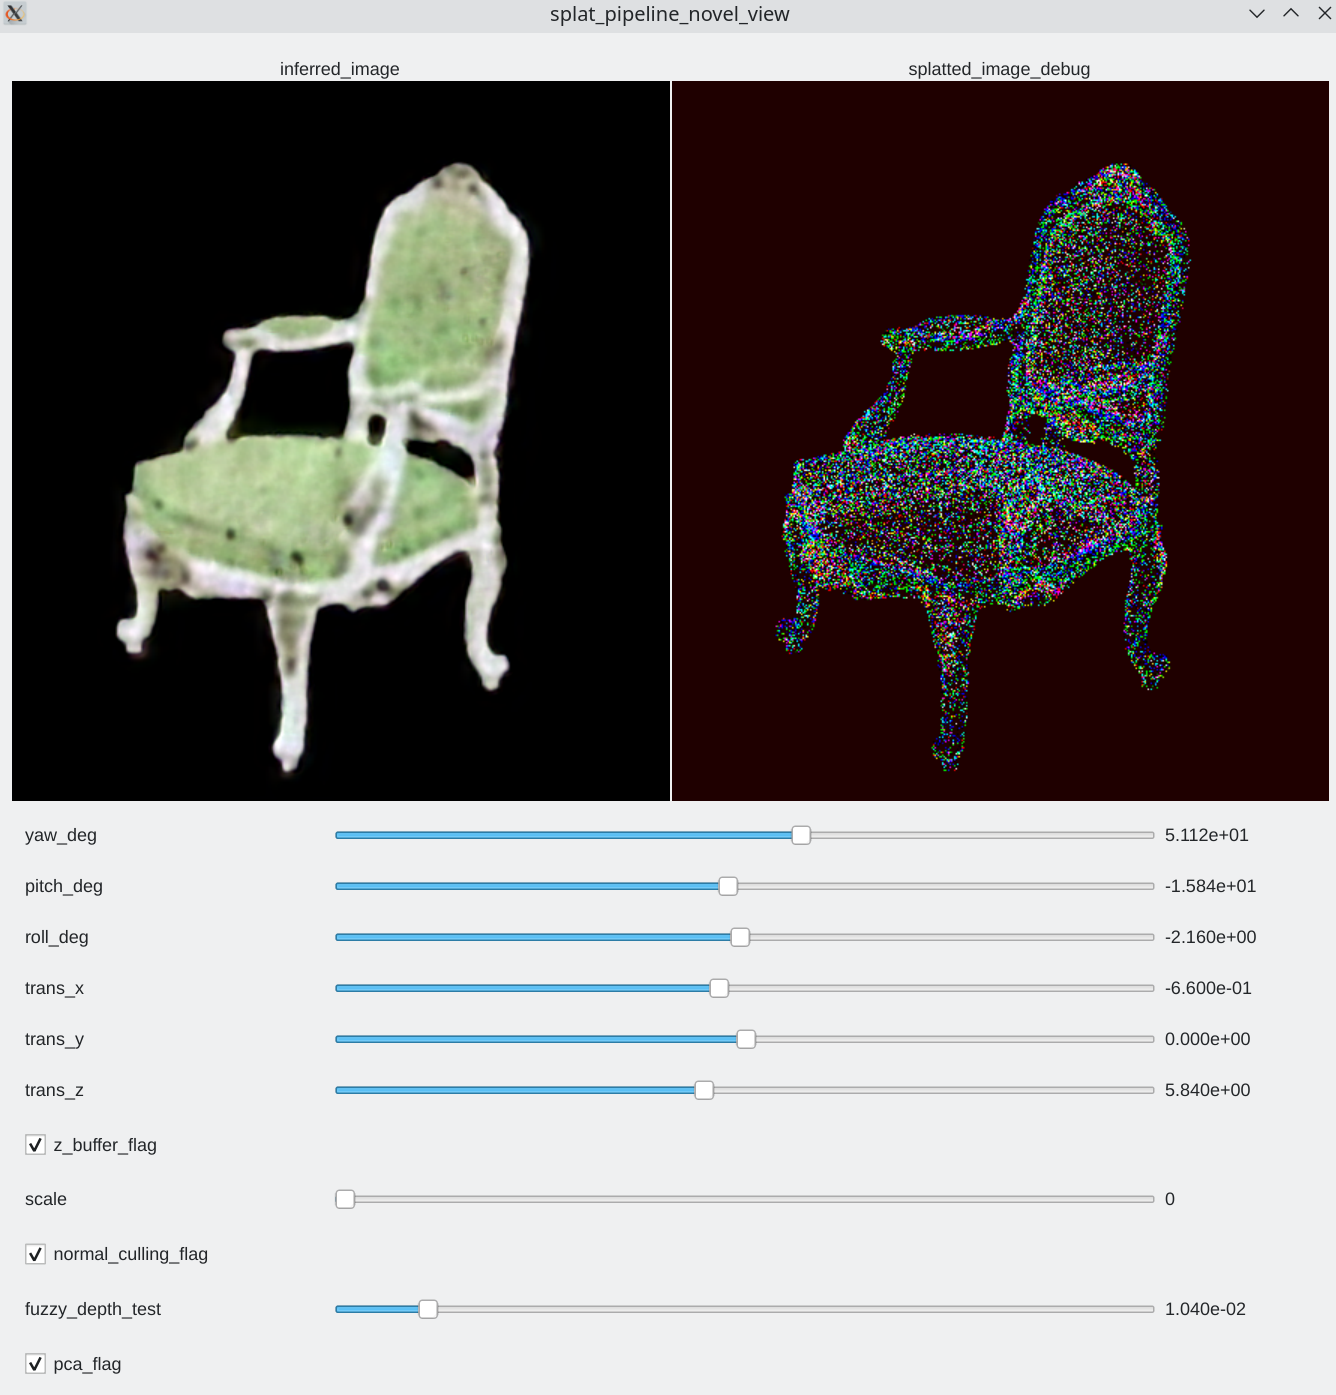
\includegraphics[width=0.45\textwidth]{figures/inference_live.png}
    \caption{Live inference, the user can move the camera around the scene and see the novel view rendered in real time. On the right side we visualize the projected pseudo colored point cloud of dimension 8 using a Principal Component Analyzis.}
    \label{fig:live_inference}
\end{figure}



\begin{table*}[htpb]
    \begin{tabular}{|l|l|l|l|l|l|}
    \hline
    Number of points & PSNR   & Mode     & Convolutions size & Pseudo color dimension & Multi-scale supervision \\ \hline
    100k             & 16.7dB & Bypass   & 1x1               & 3                      & Yes                     \\ \hline
    100k             & 21.2dB & Conv 5x5 & 5x5               & 3                      & Yes                     \\ \hline
    100k             & 26.3dB & Vanilla  & 5x5               & 8                      & No                      \\ \hline
    100k             & \textbf{29dB}   & Vanilla  & 5x5               & 8                      & Yes                     \\ \hline
    400k             & 23dB   & Bypass   & 1x1               & 3                      & No                      \\ \hline
    800k             & 25db   & Bypass   & 1x1               & 3                      & No                      \\ \hline
\end{tabular}
\caption{We report quantitative performances (PSNR on validation set) of various training configurations on the \texttt{Old chair} scene.}
\label{tab:results}
\end{table*}